\documentclass[11pt]{article}

\usepackage{graphics} % or graphicx 
\usepackage{epstopdf}
\usepackage{multirow}
\usepackage{amsmath}



\setlength{\oddsidemargin}{0in}
\setlength{\textwidth}{6.5in}
\setlength{\topmargin}{-0.5in}
\setlength{\textheight}{8.75in}
\setlength{\parindent}{0pt}
\setlength{\parskip}{6pt}

\usepackage{fancyhdr}
\pagestyle{fancy}
\lhead{HW2}
\rhead{Reza Shisheie}

\usepackage{epsfig,graphicx}

\usepackage{amsmath}

\usepackage{clrscode3e}

\begin{document}

\thispagestyle{plain}

\begin{center}
{\Large \bf CIS 606 \hfil Homework 2 \hfil Fall 2019} \\
\end{center}

\vskip 1in 

\centerline{
\includegraphics[width=3in]{photo.jpg}}

\vskip 0.5in 


\begin{center}
\begin{tabular}{ll}
{\bf Name:}     & {\bf Reza Shisheie } \\ \\
{\bf Login ID:} & {\bf reshishe }   
\end{tabular}
\end{center}

\newpage

\begin{enumerate}

\itemsep 0.35in


\item Use a drawing tool to draw figure 6.5 (c) and (d) on page 165: 

	Figure.\ref{fig:prob1-c} and \ref{fig:prob1-d} show the two figures from book:

	\begin{figure}[h!]
		\centerline{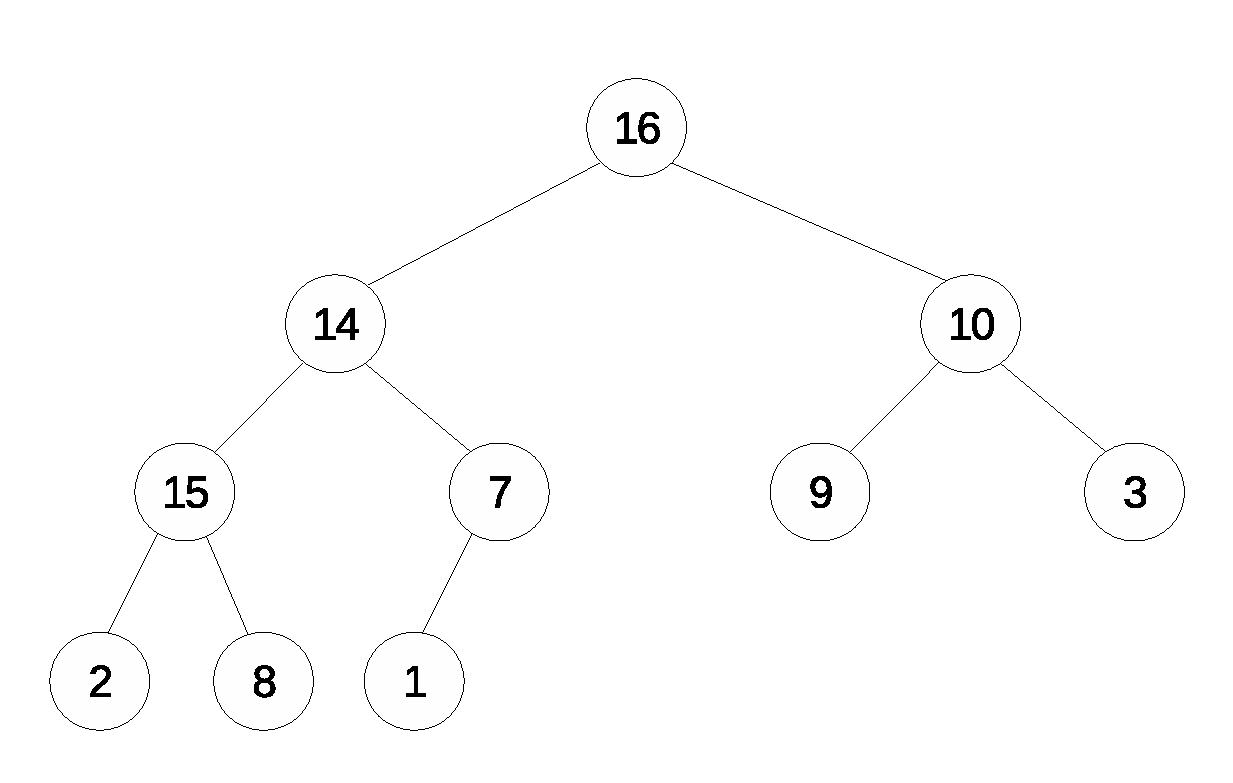
\includegraphics[width=4in]{prob1-c.eps}}
		\caption{From book, Figure 6.5 (c) on page 165}
		\label{fig:prob1-c}
	\end{figure}
	
	\begin{figure}[h!]
		\centerline{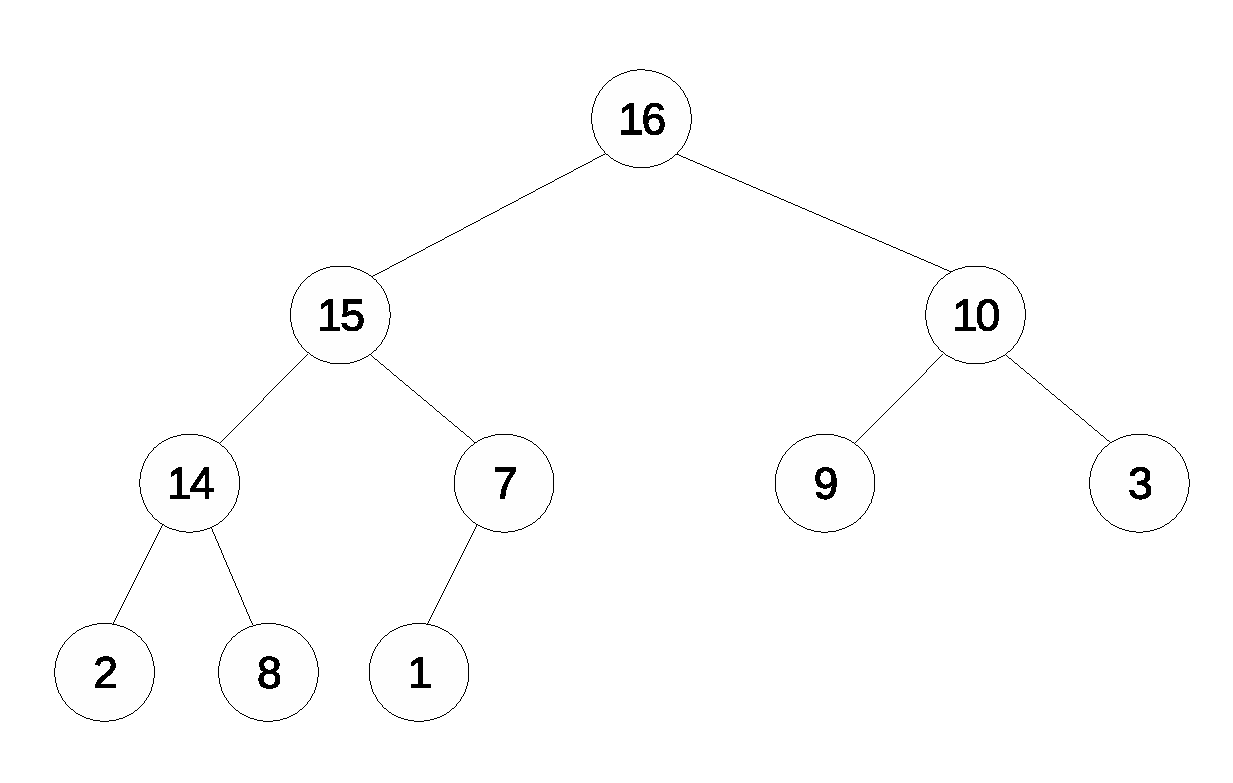
\includegraphics[width=4in]{prob1-d.eps}}
		\caption{From book, Figure 6.5 (d) on page 165}
		\label{fig:prob1-d}
	\end{figure}





\item Problem 3-4f (Textbook page 62):

	If $ f(n)= O(g(n)) $ $\implies$ $ \exists $ $ c, $ $ n_0>0 $ such that $ 0 \leq f(n) \leq cg(n) $ for all $ n \geq n_0 $  
	
	If $ g(n)= \Omega(f(n)) $ $\implies$ $ \exists $ $ c{'}, $ $ n_0>0 $ such that $ 0 \leq c{'}f(n) \leq g(n) $ for all $ n \geq n_0 $     
	
	Considering the two inequalities, if the first inequality is divided by $c$ and $c{'} = 1/c$, then second inequality is achieved. Thus, two inequalities are the same and $c{'} = 1/c$.  





\pagebreak

\item Problem 4.3-9 (Textbook page 88):
	
	$ T(n) = 3T(\sqrt[•]{n}) + \log(n) $ 
	$ \overset{n=2^m}{\implies} $ 
	$ T(2^m) = 3T(\sqrt[•]{2^m}) + \log(2^m) $ 
	$ \implies $ 
	$T(2^m) = 3T(2^{m/2}) + m $ 
	$ \overset{S(m)=T(2^m) \implies S(m/2)=T(2^{m/2})}{\implies} $ 
	$ S(m) = 3S(m/2) + m$ 
	
	
	\begin{itemize}
    	\item METHOD 1:
     	According to Figure 4.7 of textbook on page 99, the tree expansion of $ S(m) = 3S(m/2) + m$ will be like Figure.\ref{fig:prob2} in the following:
     	
		\begin{figure}[h!]
			\centerline{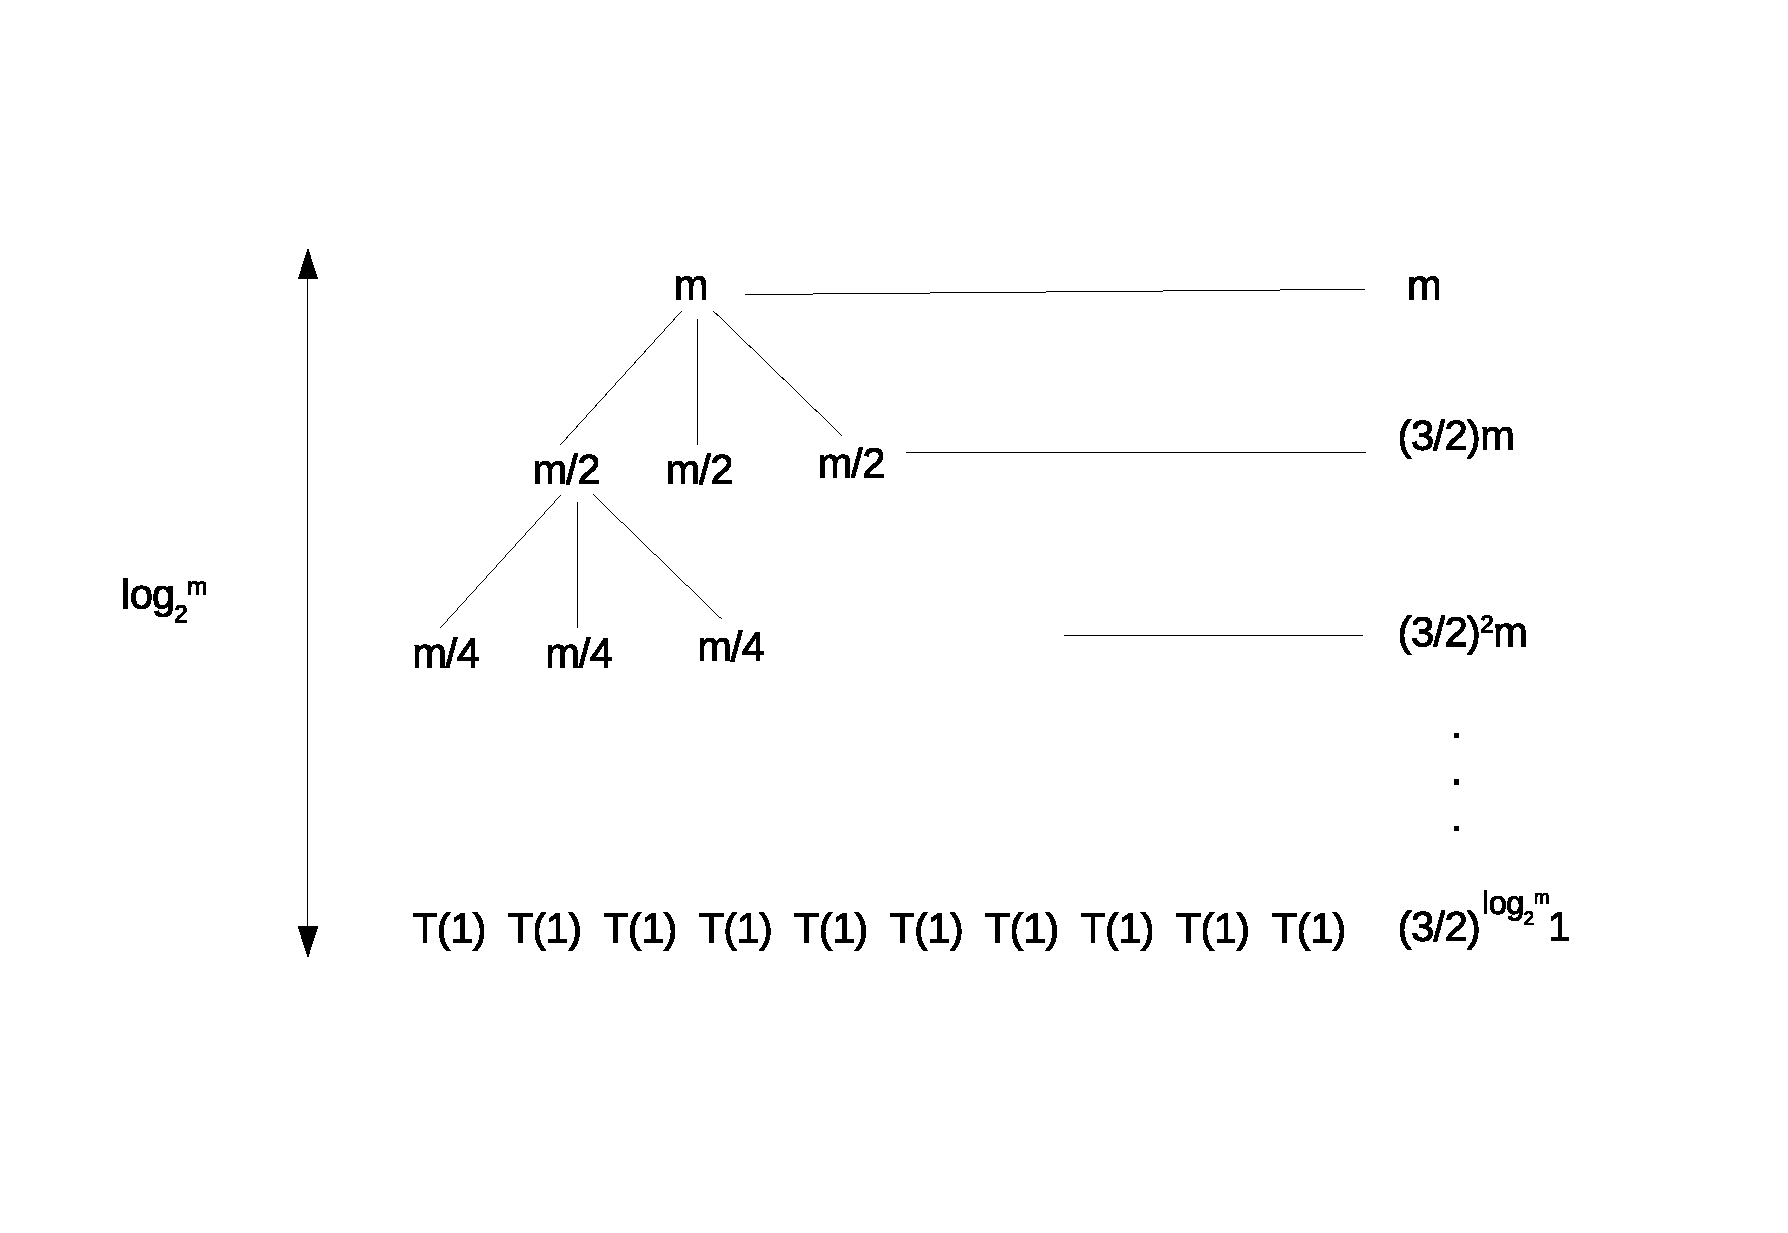
\includegraphics[width=5in]{prob2.eps}}
			\caption{Expanded tree}
			\label{fig:prob2}
		\end{figure}
	
		$S(m) = m+\frac{3}{2}m+{(\frac{3}{2})}^2m+...+{(\frac{3}{2})}^{\log_2{m-1}}m+\Theta(3^{\log_2{m}})$
		
		$S(m) = \sum_{k=0}^{\log_2{(m-1)}} {(\frac{3}{2})}^k m + \Theta(3^{\log_2{m}})  $
		
		Since $	\Theta(3^{\log_2{m}})  $ is the dominant term in the bracket (leave dominant), $S(m)$ can be simpliefied to :
		
		$S(m) = \Theta(3^{\log_2{m}}) $

		By flipping $m$ and $3$, $S(m)$ becomes:
		
		$S(m) = \Theta(m^{\log_2{3}}) $
		$\overset{m=\log_2{n}}{\implies}T(n)=\log_2{n}^{\log_3{2}}$	
	    
    \end{itemize}	
	

	\begin{itemize}
	    \item METHOD 2:
	    
	    Using Master theorem for $ S(m) = 3S(m/2) + m$ :
	    
    	$a=3$, $b=2$, $f(m)=m$
    	
    	$m^{\log_b{a}-\epsilon} \overset{}{=} m^{\log_{2}{3}-\epsilon}=m^{1.58-\epsilon}\overset{\epsilon=0.58}{=}m$  
	    $\overset{\mathrm{•}}{\implies} f(m)=O(m^{\log_b{a}-\epsilon}):\epsilon=0.58$
	    
	    $\overset{\mathrm{Case 1}}{\implies} S(m)=\Theta(m^{\log_b{a}})$	
	    $\overset{\mathrm{}}{=}T(2^m)$
	    $\overset{\mathrm{}}{=}T(n)$
	    $\overset{m=\log_2{n}}{\implies}T(n)=\log_2{n}^{\log_b{a}}$	
	    $\overset{}{\implies}$
	    
	    $T(n)=\log_2{n}^{\log_2{3}}$	
  		%$\overset{m=\log_2{n}}{\implies} T(2^{m})=T(n)=\Theta(m^{\log_b{a}})$
  		 

    \end{itemize}
    
    As you case Method 1 and Method 2 yield the same result.
	
	
	
	

	
	
	 
\pagebreak
	
\item Problem 4.5-1a (Textbook page 96):
	
	$T(n)=2T(n/4)+1$
	
	$a=2$, $b=4$, $f(n)=1$
	
	$n^{\log_b{a}-\epsilon} \overset{\epsilon=0.5}{=} n^{(\log_4{2})-0.5}=n^{0}=1
	\overset{\mathrm{•}}{\implies} f(n)=O(n^{\log_b{a}-\epsilon}):\epsilon=0.5$
	
	$\overset{\mathrm{Case 1}}{\implies} T(n)=\Theta(n^{\log_b{a}})=\Theta(n^{\log_4{2}})=\Theta(\sqrt[•]{n}) 
	\overset{\mathrm{•}}{\implies} T(n)=\Theta(\sqrt[•]{n}) $ 







\item Problem 4-1b (Textbook page 107):

	$T(n)=T(7n/10)+n$

	$a=1$, $b=10/7$, $f(n)=n$, 
	
	$n^{\log_b{a}+\epsilon} \overset{}{=} n^{\log_{10/7}{1}+\epsilon}=n^{0+\epsilon}\overset{\epsilon = 1}{=}n^{1}=n  
	\overset{}{\implies} f(n)=\Omega(n)
	\overset{}{\implies} f(n)=\Omega(n^{\log_b{a}+\epsilon}):\epsilon=1$
	
	If $c=8/10$ and $c<1 \overset{}{\implies} $
	$
	    \left\{\begin{array}{lr}
        	af(n/b)=f(7n/10)=7n/10\\
        	cf(n)=8n/10\\
        \end{array}\right\}
    $ 
    $ \overset{}{\implies} af(n/b)\leq cf(n)$
     is valid!
    
    $ \overset{\mathrm{Case 3}}{\implies} T(n)=\Theta(f(n))$
    $ \overset{}{\implies} T(n)=\Theta(n)$



\item Problem 4.1c (Textbook page 107):

	$T(n)=16T(n/4)+n^{2}$
	
	$a=16$, $b=4$, $f(n)=n^{2}$,
	
	$n^{\log_b{a}} \overset{}{=} n^{\log_{4}{16}}=n^{2}  
	\overset{}{\implies} f(n)=\Theta(n^{\log_b{a}}.\log{n})$
	
	$	\overset{\mathrm{Case 2}}{\implies} f(n)=\Theta(n^{2}.\log{n})$
	
	























   
\end{enumerate}

\end{document}

